\documentclass[a4paper, titlepage]{jsarticle}

\usepackage[dvipdfmx]{graphicx}
\usepackage{amsmath}
\usepackage{mathtools}
\usepackage{listings}

\lstset{
  basicstyle={\ttfamily},
  identifierstyle={\small},
  commentstyle={\smallitshape},
  keywordstyle={\small\bfseries},
  ndkeywordstyle={\small},
  stringstyle={\small\ttfamily},
  frame={tb},
  breaklines=true,
  columns=[l]{fullflexible},
  numbers=left,
  xrightmargin=0zw,
  xleftmargin=3zw,
  numberstyle={\scriptsize},
  stepnumber=1,
  numbersep=1zw,
  lineskip=-0.5ex
}

\title{シミュレーション工学Ⅱ ヤコビ法,ガウス・ザイデル法}
\author{三浦夢生}
\date{2020}

\begin{document}
	\maketitle

	\section{反復法}
	与えられた方程式に対して,ガウスの消去法やLU分解といった有限回の手順を踏んで代数的に厳密に解く直接法に対して,ヤコビ法やガウス・ザイデル法などは反復法と呼ばれ,与えられた初期値からある収束する解を近似的に求める方法である.
	反復法は直接法に比べてメモリの使用量,計算量が少なく済む反面,終了条件の影響が大きい,収束しないことがあるといった短所もある.

	\section{ヤコビ法}
	与えられた連立一次方程式
	
		\begin{align}
			\left(
				\begin{array}{cccc}
					{a_{11}} & {a_{12}} & {\ldots} & {a_{1n}} \\
					{a_{21}} & {a_{22}} & {\ldots} & {a_{2n}} \\
					{\vdots} & {\vdots} & {\ddots} & {\vdots} \\
					{a_{n1}} & {a_{n2}} & {\ldots} & {a_{nn}}
				\end{array}
			\right)
			\left(
				\begin{array}{cccc}
					{x_{1}} \\
					{x_{2}} \\
					{\vdots} \\
					{x_{n}}
				\end{array}
			\right)
			%
			=
			%
			\left(
				\begin{array}{cccc}
					{b_{1}} \\
					{b_{2}} \\
					{\vdots} \\
					{b_{n}}
				\end{array}
			\right)
		\end{align}

	に対して解を

		\begin{equation}
			{{x_{i}}^{(k*1)}} = {\frac{1}{a_{ii}}}({b_{i}} - {a_{i1}}{{x_{1}}^{(k)}} - {a_{i2}}{{x_{2}}^{(k)}} - {\cdots} - {a_{ii-1}}{{x_{i-1}}^{(k)}} - {a_{ii+1}}{{x_{i+1}}^{(k)}} - {\cdots} - {a_{in}}{{x_{n}}^{(k)}})
		\end{equation}

	とし,初期値${{x_{i}}^{0}}$と終了条件を与えて一つずつ解を計算する.終了条件はしばしば$|{{x_{i}}^{(k+1)}} - {{x_{i}}^{(k)}}| < {\epsilon}$とされる.ここで${\epsilon}$は精度を決める定数である.

	\section{ガウス・ザイデル法}
	概ねヤコビ法と同様であるが,解の求め方に違いがある.ヤコビ法では解を一つずつ求めていたが,ガウス・ザイデル法では以下のようにする.右辺の変数を常に最新の値を用いて計算する.

		\begin{eqnarray}
			&{{x_{1}}^{(k+1)}} = {\frac{1}{a_{11}}}({b_{1}} - {a_{12}}{{x_{2}}^{(k)}} - {a_{13}}{{x_{3}}^{(k)}} - {a_{14}}{{x_{4}}^{(k)}} - {\cdots} - {a_{1n}}{{x_{n}}^{(k)}}) \nonumber \\
			&{{x_{2}}^{(k+1)}} = {\frac{1}{a_{22}}}({b_{2}} - {a_{21}}{{x_{1}}^{(k+1)}} - {a_{23}}{{x_{3}}^{(k)}} - {a_{24}}{{x_{4}}^{(k)}} - {\cdots} - {a_{2n}}{{x_{n}}^{(k)}}) \nonumber \\
			&{{x_{3}}^{(k+1)}} = {\frac{1}{a_{33}}}({b_{3}} - {a_{31}}{{x_{1}}^{(k+1)}} - {a_{32}}{{x_{2}}^{(k+1)}} - {a_{34}}{{x_{4}}^{(k)}} - {\cdots} - {a_{3n}}{{x_{n}}^{(k)}}) \nonumber \\
			&{\vdots} \\
			&{{x_{n}}^{(k+1)}} = {\frac{1}{a_{nn}}}({b_{n}} - {a_{n1}}{{x_{1}}^{(k+1)}} - {a_{n2}}{{x_{2}}^{(k+1)}} - {a_{n3}}{{x_{3}}^{(k+1)}} - {\cdots} - {a_{nn-1}}{{x_{n-1}}^{(k+1)}})
		\end{eqnarray}

	\section{手計算}
	$k=3$まで手計算を行った画像を付録6.5に示す.

	今回手計算の労力を加味し,小数第5位までで計算を行った.

	アルゴリズムの理解の助けになり,実装する際にも役立った.

	\section{実行結果}
	実行回数をともに20回に設定し,x成分の変化を表したグラフを以下に示す.

			\begin{figure}[ht]
				\begin{tabular}{cc}
					\begin{minipage}[t]{10cm}
						\centering
						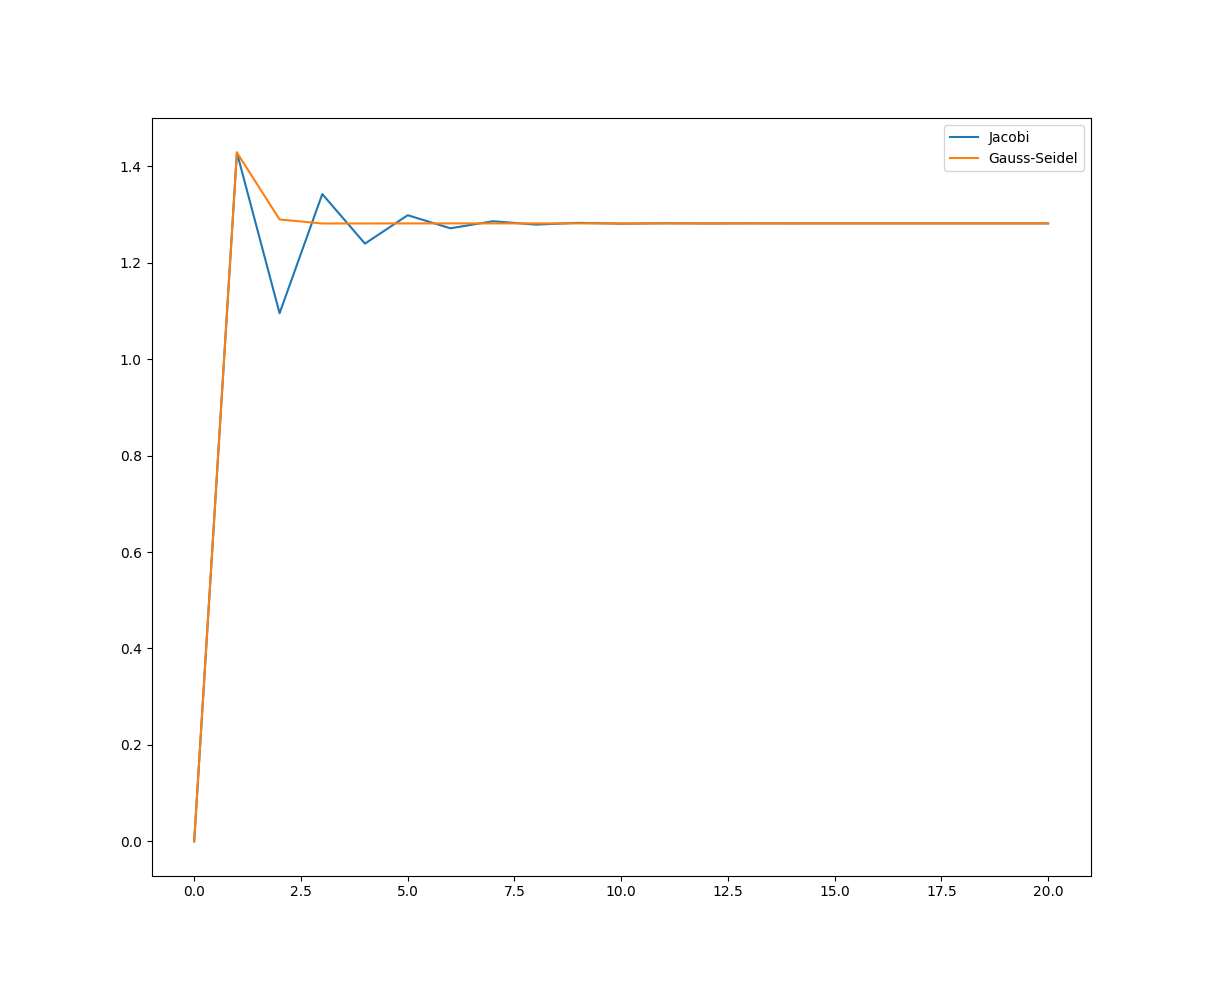
\includegraphics[keepaspectratio, scale=0.5]{compareX.png}
					\end{minipage}
				\end{tabular}
			\end{figure}

	この場合どちらも試行回数10回目までには収束しており,またヤコビ法よりもガウス・ザイデル法のほうが収束が早いことがわかる.

	グラフからもわかるが,試行回数が少ないと収束しないが多すぎても無駄な計算になってしまうことを確認した.

	またヤコビ法,ガウス・ザイデル法で終了条件を満たすまで計算を続けた結果をそれぞれ以下に示す.ただし,終了条件は前後の差の絶対値が${\epsilon = 10^{-7}}$となるまでとした.

		
		\begin{lstlisting}
% python3 JacobiMethod.py 
x=1.4285714285714286, y=1.0, z=0.6666666666666666 / count=1
x=1.0952380952380953, y=0.5714285714285714, z=0.015873015873015817 / count=2
x=1.342403628117914, y=0.8571428571428572, z=0.23280423280423276 / count=3
x=1.2396069538926682, y=0.7448979591836735, z=0.0826404635928445 / count=4
x=1.2985458733758055, y=0.8140589569160998, z=0.14289913496262704 / count=5
x=1.271448967594092, y=0.7840945902170392, z=0.10674793138889882 / count=6
x=1.2860585067150232, y=0.8010384047799014, z=0.1227575882400776 / count=7
x=1.2790637741057063, y=0.793208591070593, z=0.11386308580336103 / count=8
x=1.282723605331812, y=0.7974183710605263, z=0.11802740873075655 / count=9
x=1.2809324016397086, y=0.7953992710594898, z=0.11581085290608861 / count=10
x=1.2818541461611905, y=0.7964543799552533, z=0.11688193150467925 / count=11
x=1.2813973938621983, y=0.7959375074155964, z=0.11632539642353991 / count=12
x=1.2816302428196178, y=0.7962033021083977, z=0.1165991877809793 / count=13
x=1.2815140460470917, y=0.7960715242296805, z=0.11645884533728573 / count=14
x=1.2815729692993927, y=0.7961386772426313, z=0.11652859280186394 / count=15
x=1.2815434481648058, y=0.796105156536877, z=0.11649311440814675 / count=16
x=1.2815583735209757, y=0.7961221510763442, z=0.11651084822886196 / count=17
x=1.2815508789237045, y=0.7961136352240548, z=0.1165018666365574 / count=18
x=1.2815546616432614, y=0.7961179401458279, z=0.11650637072004738 / count=19
x=1.2815527597734397, y=0.7961157782745746, z=0.11650409514177706 / count=20
x=1.2815537187774102, y=0.7961168693501537, z=0.11650523840326629 / count=21
x=1.2815532362633306, y=0.7961163207515989, z=0.11650466159941313 / count=22
x=1.2815534794356533, y=0.7961165973673038, z=0.1165049516909491 / count=23
x=1.2815533570358284, y=0.7961164581864374, z=0.1165048054474202 / count=24
x=1.2815534187026747, y=0.7961165283277389, z=0.11650487904100339 / count=25
calc 25 times.
		\end{lstlisting}
		
		\begin{lstlisting}
% python3 GaussSeidelMethod.py
x=1.4285714285714286, y=0.8214285714285714, z=0.07539682539682542 / count=1
x=1.2896825396825398, y=0.810515873015873, z=0.10989858906525571 / count=2
x=1.2813838498362309, y=0.7986150478710002, z=0.11570968407939307 / count=3
x=1.281423654852888, y=0.7964309116136166, z=0.11642888393926379 / count=4
x=1.2815301886439794, y=0.7961478949422787, z=0.11649954865391167 / count=5
x=1.281550429678557, y=0.7961188655449635, z=0.1165047271119995 / count=6
x=1.2815530971758626, y=0.7961165901860173, z=0.11650489278780254 / count=7
x=1.2815533748911967, y=0.7961164933431745, z=0.11650486335423141 / count=8
x=1.2815533971354804, y=0.7961165016002282, z=0.116504855658706 / count=9
calc 9 times.
		\end{lstlisting}

	このように,ヤコビ法よりもガウス・ザイデル法のほうが収束が早く,計算する回数が少なくて済むことがわかる.終了条件を$10^{-9}$や$10^{-12}$などに変えてみても,ガウス・ザイデル法のほうが早く収束することを確認した.

	\section{付録}
	今回行った手計算の画像及び作成したソースコードを以下に示す.

		\subsection{ヤコビ法 プログラム1}
			\begin{lstlisting}
import numpy as np

def Jacobi_method(x0, y0, z0, A, b):
    EPSILON = 1.0e-7
    x_t = x0
    y_t = y0
    z_t = z0
    cnt = 0
    
    x = 0
    y = 0
    z = 0
    
    X = [x]
    Y = [y]
    Z = [z]

    '''
    for i in range(20):
	x = (b[0] - (A[0][1] * y_t + A[0][2] * z_t)) / A[0][0]
	y = (b[1] - (A[1][0] * x_t + A[1][2] * z_t)) / A[1][1]
	z = (b[2] - (A[2][0] * x_t + A[2][1] * y_t)) / A[2][2]
	X.append(x)
	Y.append(y)
	Z.append(z)
	x_t = x
	y_t = y
	z_t = z
    '''

    while True:
	cnt += 1
	x = (b[0] - (A[0][1] * y_t + A[0][2] * z_t)) / A[0][0]
	y = (b[1] - (A[1][0] * x_t + A[1][2] * z_t)) / A[1][1]
	z = (b[2] - (A[2][0] * x_t + A[2][1] * y_t)) / A[2][2]
	X.append(x)
	Y.append(y)
	Z.append(z)
	print(f'x={x}, y={y}, z={z} / count={cnt}')
	if np.abs(x - x_t) < EPSILON and np.abs(y - y_t) < EPSILON and np.abs(z - z_t) < EPSILON:
	    break
	x_t = x
	y_t = y
	z_t = z
    print(f'calc {cnt} times.')

    return X, Y, Z, cnt

if __name__ == '__main__':
    A = np.array([[7, 1, 2],
		[1, 8, 3],
		[2, 3, 9]], dtype=float)
    b = np.array([10, 8, 6], dtype=float)

    x0 = 0
    y0 = 0
    z0 = 0

    X, Y, Z, cnt = Jacobi_method(x0, y0, z0, A, b)
			\end{lstlisting}

		\subsection{ヤコビ法 プログラム2}
			\begin{lstlisting}
import numpy as np

def Jacobi_method(A, b, x_init):
    EPSILON = 1.0e-7
    x_t = x_init
    size = len(x_t)
    flag = 0
    cnt = 0

    x = np.zeros(size, dtype=float)

    '''
    for time in range(10):
	for i in range(size):
	    s = 0
	    for j in range(size):
		if i != j:
		    s += A[i][j] * x_t[j]
	    x[i] = (b[i] - s) / A[i][i]
	for i in range(size):
	    x_t[i] = x[i]
    '''

    while True:
	cnt += 1
	#
	# calculation
	#
	for i in range(size):
	    s = 0
	    for j in range(size):
		if i != j:
		    s += A[i][j] * x_t[j]
	    x[i] = (b[i] - s) / A[i][i]
	#
	# Exit conditions
	#
	flag = 0
	for i in range(size):
	    if np.abs(x[i] - x_t[i]) < EPSILON:
		flag += 1
	if flag == size:
	    break
	#
	# update value
	#
	for i in range(size):
	    x_t[i] = x[i]
    print(f'calc {cnt} times.')

    return x

if __name__ == '__main__':
    A = np.array([[7, 1, 2],
		[1, 8, 3],
		[2, 3, 9]], dtype=float)
    b = np.array([10, 8, 6], dtype=float)
    x_init = np.array([0, 0, 0], dtype=float)

    x = Jacobi_method(A, b, x_init)

    for i in range(len(x)):
	print(f'x[{i}] = {x[i]}')
			\end{lstlisting}

		\subsection{ガウス・ザイデル法 プログラム1}
			\begin{lstlisting}
import numpy as np

def GaussSeidel_method(x0, y0, z0, A, b):
    EPSILON = 1.0e-7
    x_t = x0
    y_t = y0
    z_t = z0
    cnt = 0
    
    x = 0
    y = 0
    z = 0
    
    X = [x]
    Y = [y]
    Z = [z]

    '''
    for i in range(20):
	x = (b[0] - (A[0][1] * y + A[0][2] * z)) / A[0][0]
	y = (b[1] - (A[1][0] * x + A[1][2] * z)) / A[1][1]
	z = (b[2] - (A[2][0] * x + A[2][1] * y)) / A[2][2]
	X.append(x)
	Y.append(y)
	Z.append(z)
	x_t = x
	y_t = y
	z_t = z
    '''

    while True:
	cnt += 1
	x = (b[0] - (A[0][1] * y + A[0][2] * z)) / A[0][0]
	y = (b[1] - (A[1][0] * x + A[1][2] * z)) / A[1][1]
	z = (b[2] - (A[2][0] * x + A[2][1] * y)) / A[2][2]
	X.append(x)
	Y.append(y)
	Z.append(z)
	print(f'x={x}, y={y}, z={z} / count={cnt}')
	if np.abs(x - x_t) < EPSILON and np.abs(y - y_t) < EPSILON and np.abs(z - z_t) < EPSILON:
	    break
	x_t = x
	y_t = y
	z_t = z
    print(f'calc {cnt} times.')

    return X, Y, Z, cnt

if __name__ == '__main__':
    A = np.array([[7, 1, 2],
		[1, 8, 3],
		[2, 3, 9]], dtype=float)
    b = np.array([10, 8, 6], dtype=float)

    x0 = 0
    y0 = 0
    z0 = 0

    X, Y, Z, cnt = GaussSeidel_method(x0, y0, z0, A, b)
			\end{lstlisting}

		\subsection{ガウス・ザイデル法 プログラム2}
			\begin{lstlisting}
import numpy as np

def GaussSeidel_method(A, b, x_init):
    EPSILON = 1.0e-7
    x_t = x_init
    size = len(x_t)
    flag = 0
    cnt = 0

    x = np.zeros(size, dtype=float)
    
    '''
    for time in range(10):
        for i in range(size):
            s = 0
            for j in range(size):
                if i != j:
                    s += A[i][j] * x[j]
            x[i] = (b[i] - s) / A[i][i]
        for i in range(size):
            x_t[i] = x[i]
    '''

    while True:
        cnt += 1
        #
        # calculation
        #
        for i in range(size):
            s = 0
            for j in range(size):
                if i != j:
                    s += A[i][j] * x[j]
            x[i] = (b[i] - s) / A[i][i]
        #
        # Exit conditions
        #
        flag = 0
        for i in range(size):
            if np.abs(x[i] - x_t[i]) < EPSILON:
                flag += 1
        if flag == size:
            break
        #
        # update value
        #
        for i in range(size):
            x_t[i] = x[i]
    print(f'calc {cnt} times.')

    return x

if __name__ == '__main__':
    A = np.array([[7, 1, 2],
                [1, 8, 3],
                [2, 3, 9]], dtype=float)
    b = np.array([10, 8, 6], dtype=float)
    x_init = np.array([0, 0, 0], dtype=float)

    x = GaussSeidel_method(A, b, x_init)

    for i in range(len(x)):
        print(f'x[{i}] = {x[i]}')
			\end{lstlisting}

		\subsection{手計算}
			\begin{figure}[ht]
				\begin{tabular}{cc}
					\begin{minipage}[t]{8.2cm}
						\centering
						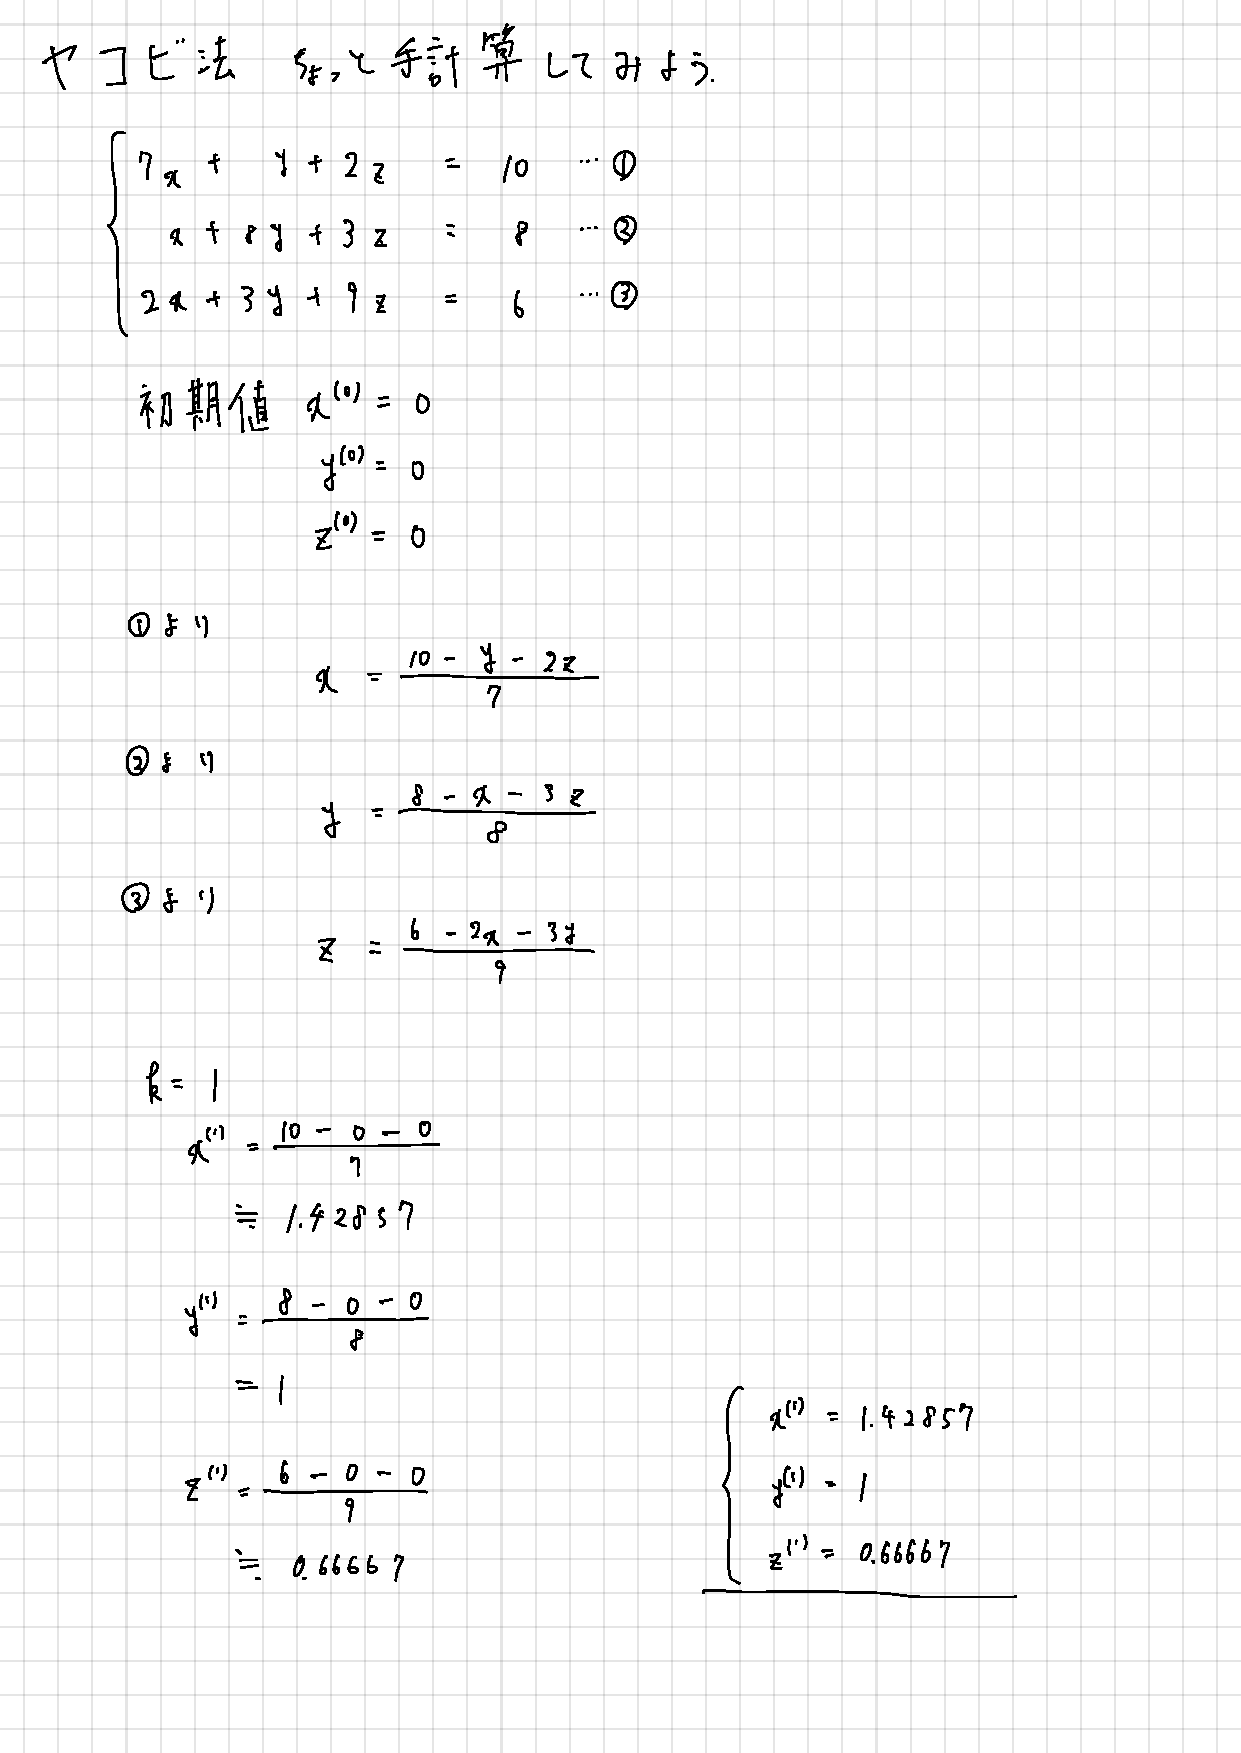
\includegraphics[keepaspectratio, scale=0.4]{Jacobi_1.pdf}
					\end{minipage} &
					\begin{minipage}[t]{8.2cm}
						\centering
						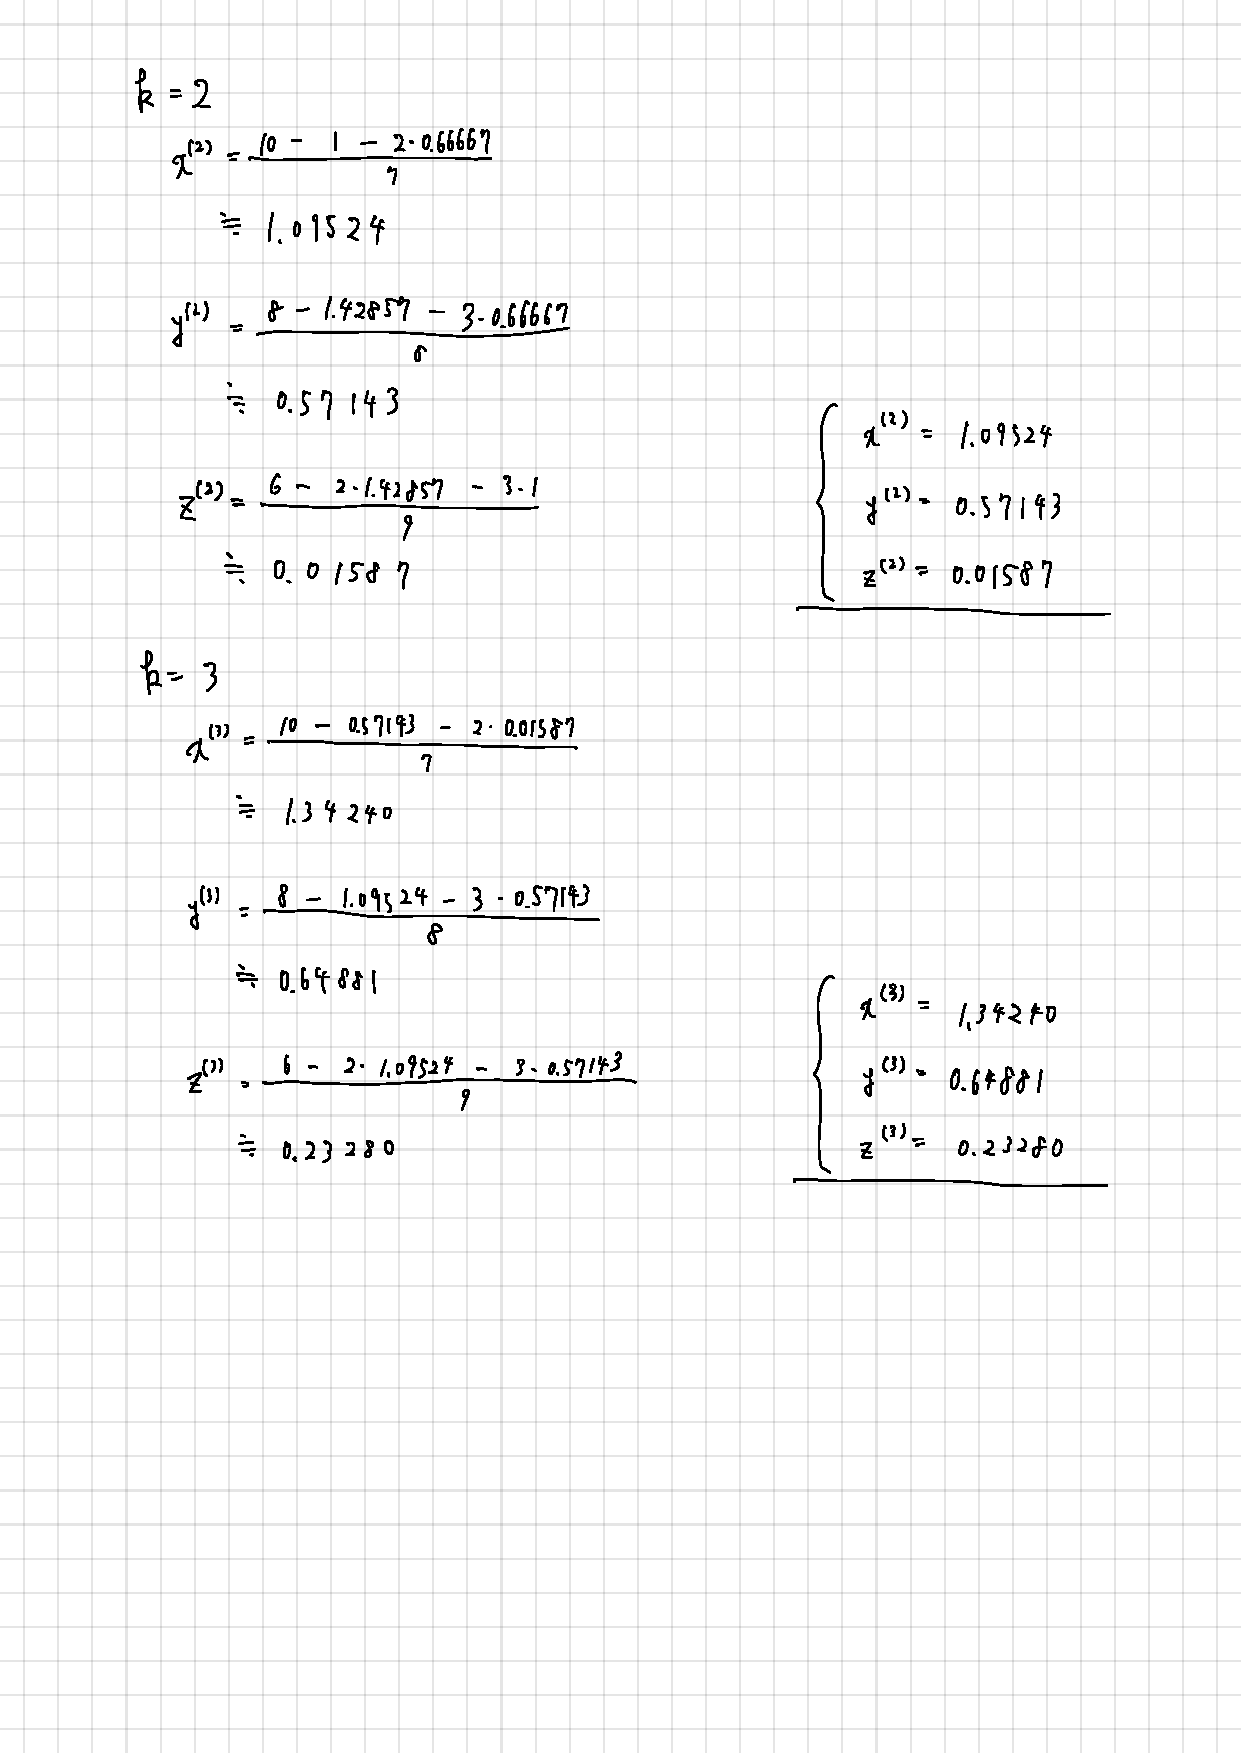
\includegraphics[keepaspectratio, scale=0.4]{Jacobi_2.pdf}
					\end{minipage} \\
					\begin{minipage}[t]{8.2cm}
						\centering
						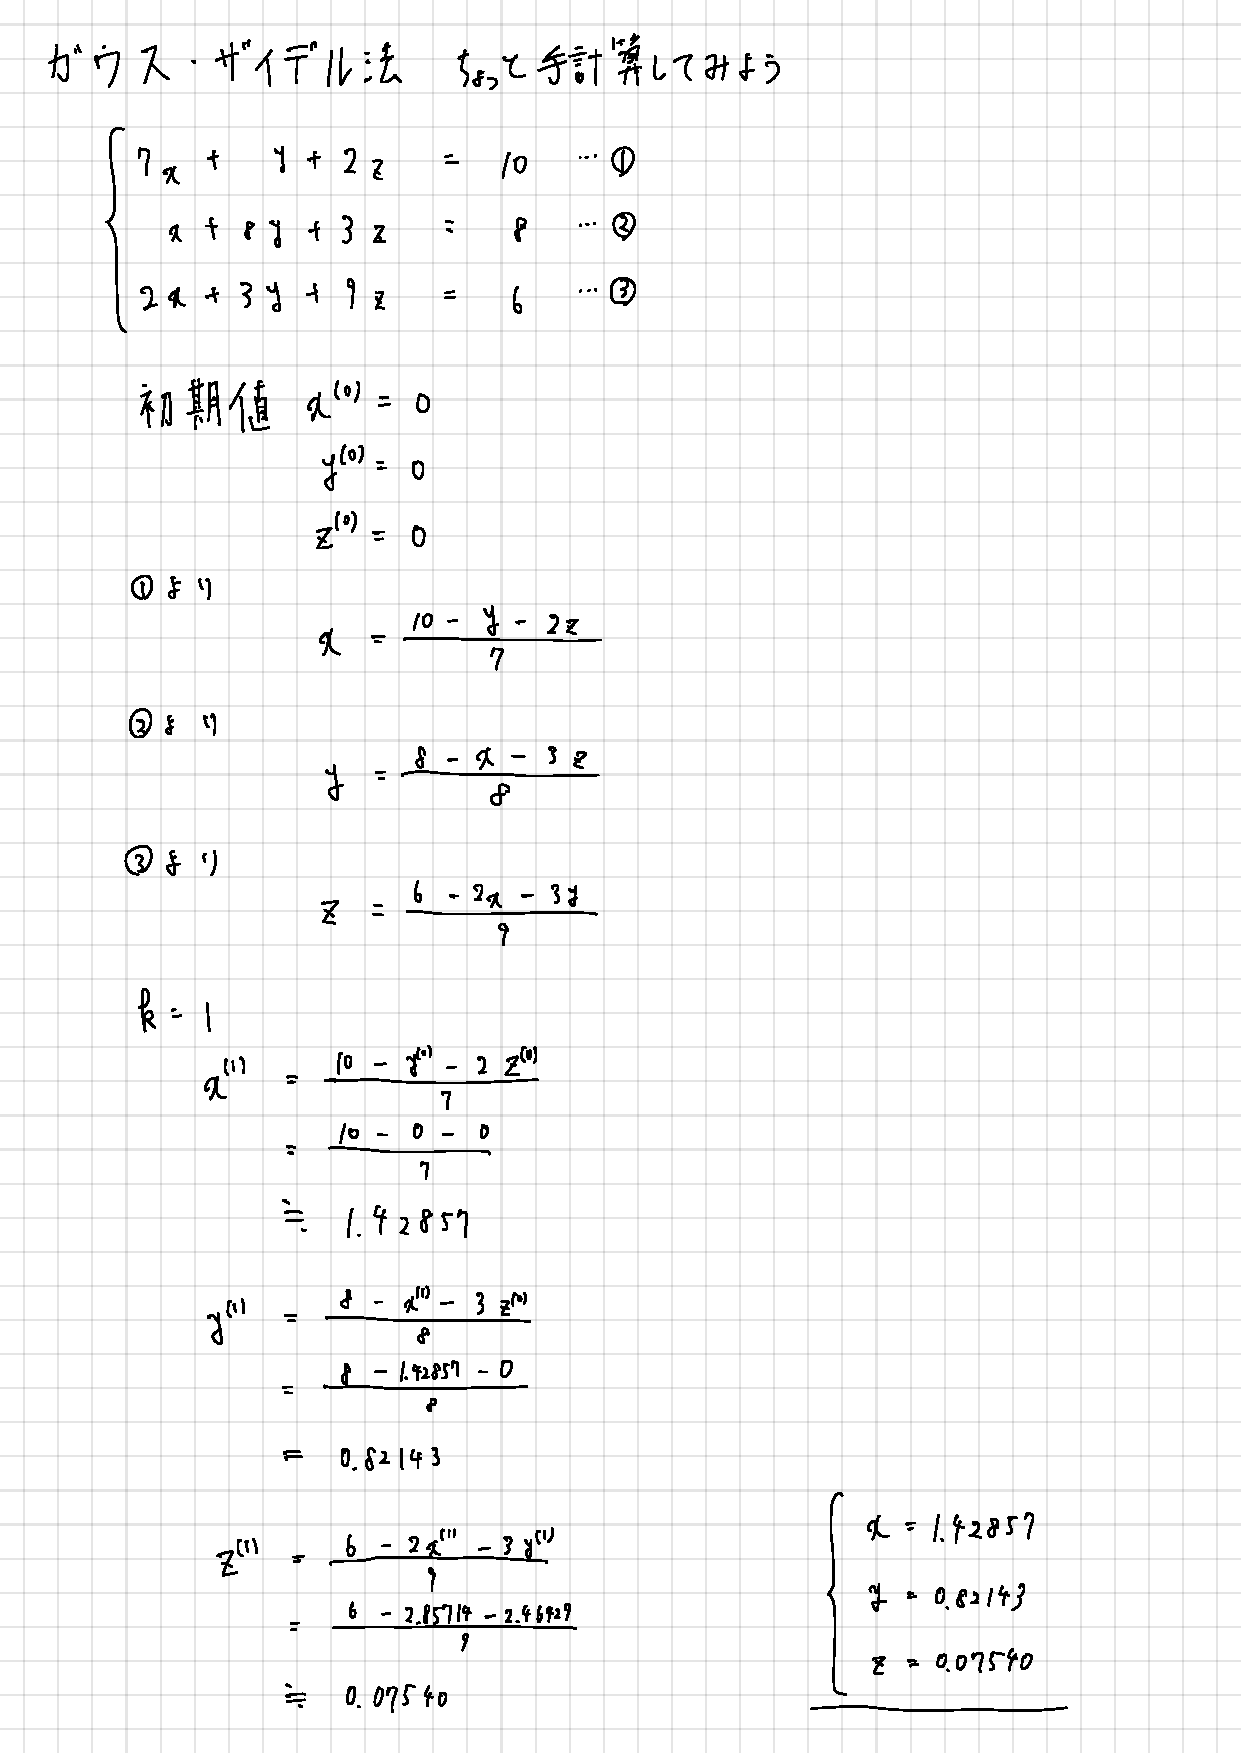
\includegraphics[keepaspectratio, scale=0.4]{GaussSeidel_1.pdf}
					\end{minipage} &
					\begin{minipage}[t]{8.2cm}
						\centering
						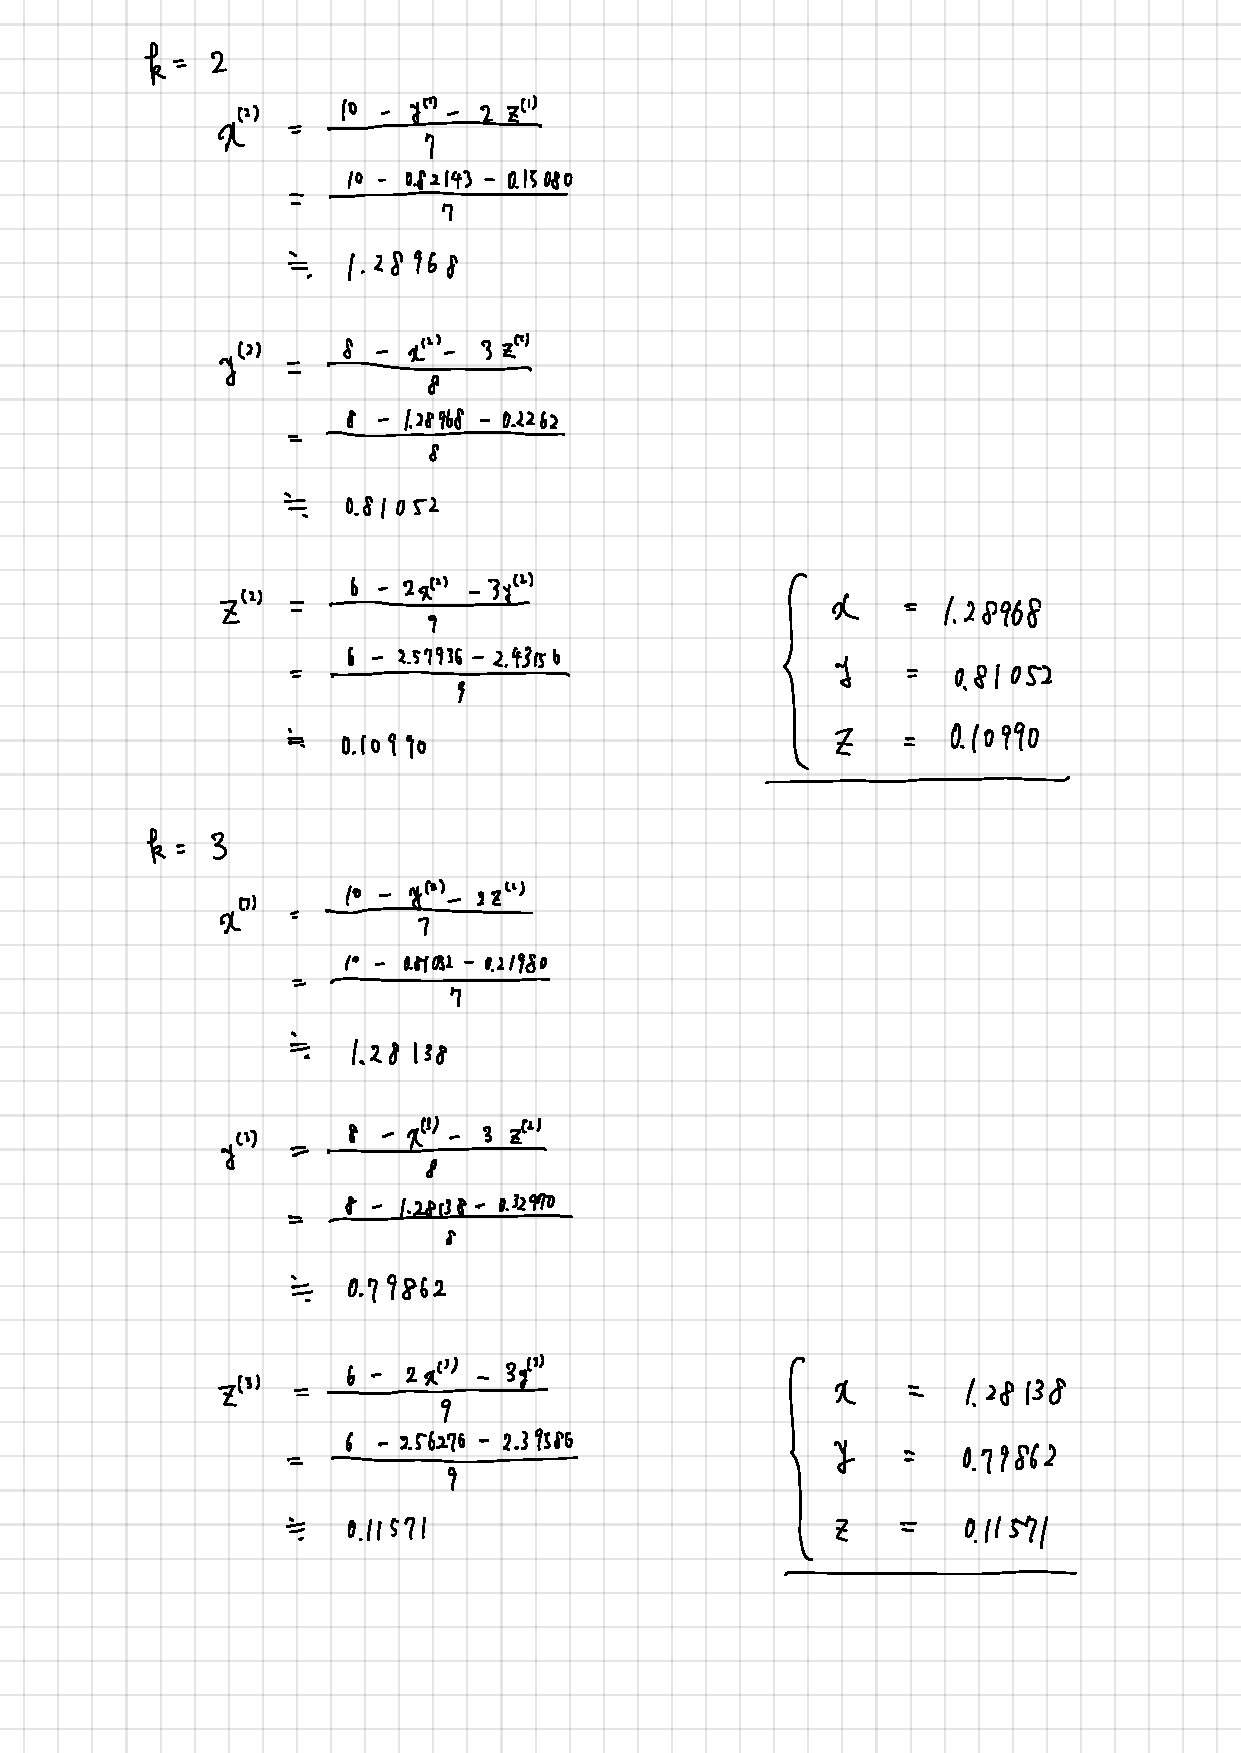
\includegraphics[keepaspectratio, scale=0.4]{GaussSeidel_2.pdf}
					\end{minipage}
				\end{tabular}
			\end{figure}

\end{document}
